\documentclass[conference]{IEEEtran}

\usepackage[utf8]{inputenc}
\usepackage{cite}
\usepackage{amsmath,amssymb,amsfonts}
\usepackage{graphicx}
\usepackage{xcolor}
\usepackage{tikz}
\usetikzlibrary{shapes.geometric, arrows.meta, positioning, fit, calc, backgrounds, patterns, circuits.logic.US, shapes.misc}
\usepackage{pgfplots}
\pgfplotsset{compat=1.17}
\usepackage{subcaption}
\usepackage{booktabs}

% Hardware component styles - PROPERLY SIZED
\tikzset{
    register/.style={
        rectangle,
        draw=black,
        thick,
        minimum width=1cm,
        minimum height=0.7cm,
        fill=white,
        font=\tiny\ttfamily
    },
    mux/.style={
        trapezium,
        trapezium left angle=70,
        trapezium right angle=110,
        draw=black,
        thick,
        minimum width=0.7cm,
        minimum height=0.6cm,
        fill=white,
        font=\tiny
    },
    alu/.style={
        rectangle,
        draw=black,
        thick,
        minimum width=0.9cm,
        minimum height=0.8cm,
        fill=white,
        font=\tiny
    },
    memory/.style={
        rectangle,
        draw=black,
        very thick,
        minimum width=0.9cm,
        minimum height=1cm,
        fill=white,
        font=\tiny
    },
    wire/.style={
        draw=black,
        thick,
        -Stealth
    },
    bus/.style={
        draw=black,
        line width=1.2pt,
        -Stealth
    },
    controlwire/.style={
        draw=black,
        dashed,
        -Stealth
    },
    buswidth/.style={
        font=\tiny,
        fill=white,
        inner sep=0.5pt
    },
    logic/.style={
        rectangle,
        draw=black,
        thick,
        rounded corners=2pt,
        minimum width=0.7cm,
        minimum height=0.6cm,
        fill=gray!10,
        font=\tiny
    },
    sbox/.style={
        rectangle,
        draw=black,
        thick,
        minimum width=0.55cm,
        minimum height=0.55cm,
        fill=gray!20,
        font=\tiny
    }
}

\begin{document}

\title{AES-128 Hardware Architecture:\\RTL Implementation on FPGA}

\author{\IEEEauthorblockN{Hardware Implementation}
\IEEEauthorblockA{Register-Transfer Level Design}}

\maketitle

%==============================================================================
% Figure 1: Complete Datapath - IMPROVED SPACING
%==============================================================================
\begin{figure*}[!t]
\centering
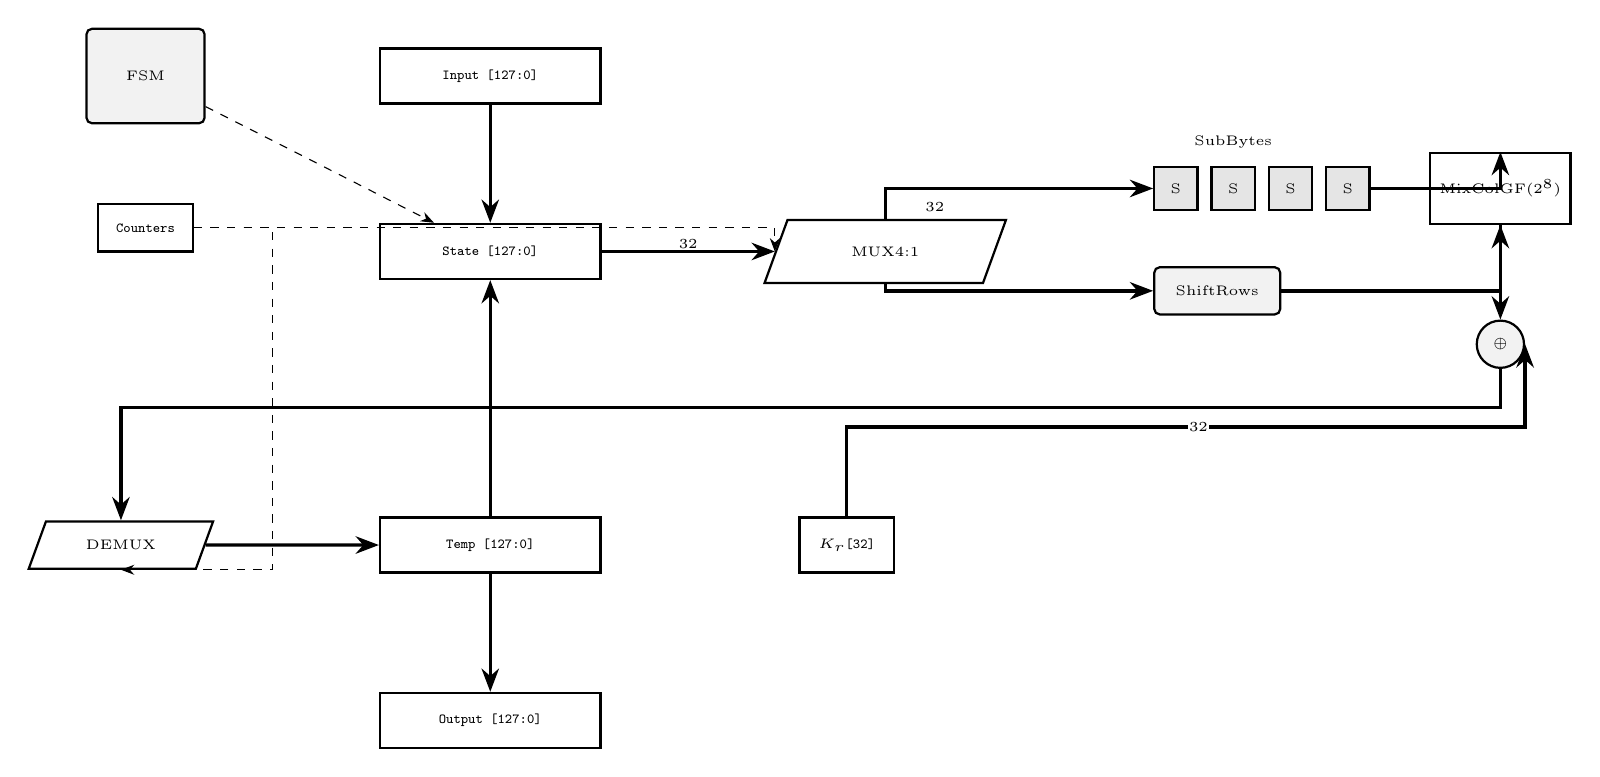
\begin{tikzpicture}[node distance=1.2cm and 1.8cm]

% State registers (left column)
\node[register, minimum width=2.8cm] (input_reg) at (0,0) {Input [127:0]};
\node[register, minimum width=2.8cm, below=1.5cm of input_reg] (state_reg) {State [127:0]};
\node[register, minimum width=2.8cm, below=3cm of state_reg] (temp_reg) {Temp [127:0]};

% Column select MUX
\node[mux, right=2.2cm of state_reg, minimum width=1.1cm, minimum height=0.8cm] (col_mux) {MUX\\4:1};
\node[buswidth, above right=0.1cm of col_mux] {32};

% Processing units (middle)
\node[sbox, right=2cm of col_mux, yshift=0.8cm] (sbox0) {S};
\node[sbox, right=0.15cm of sbox0] (sbox1) {S};
\node[sbox, right=0.15cm of sbox1] (sbox2) {S};
\node[sbox, right=0.15cm of sbox2] (sbox3) {S};
\node[font=\tiny, above=0.1cm of sbox1.north] {SubBytes};

\node[logic, right=2cm of col_mux, yshift=-0.5cm, minimum width=1.6cm] (shift) {ShiftRows};

\node[alu, right=2.2cm of sbox1, minimum width=1.4cm, minimum height=0.9cm] (mixcol) {MixCol\\GF($2^8$)};

% AddRoundKey XOR
\node[logic, circle, minimum size=0.6cm, below=1.2cm of mixcol] (xor) {$\oplus$};

% Demux back to state
\node[mux, left=2.2cm of temp_reg, shape border rotate=180, minimum width=1cm] (demux) {DEMUX};

% Key path (right side)
\node[register, right=2.5cm of temp_reg, minimum width=1.2cm] (key_word) {$K_r$[32]};

% Output register
\node[register, minimum width=2.8cm, below=1.5cm of temp_reg] (output_reg) {Output [127:0]};

% Control (top left)
\node[logic, left=2.2cm of input_reg, minimum width=1.5cm, minimum height=1.2cm] (fsm) {FSM};
\node[register, below=1cm of fsm, minimum width=1.2cm, minimum height=0.6cm] (cnt) {Counters};

% Data connections
\draw[bus] (input_reg) -- (state_reg);
\draw[bus] (state_reg) -- node[buswidth, above] {32} (col_mux);
\draw[bus] (col_mux.north) |- (sbox0.west);
\draw[bus] (sbox3.east) -| (mixcol.north);
\draw[bus] (col_mux.south) |- (shift.west);
\draw[bus] (shift.east) -| (mixcol.south);
\draw[bus] (mixcol) -- (xor);
\draw[bus] (xor) -- ++(0,-0.8) -| (demux);
\draw[bus] (demux) -- (temp_reg);
\draw[bus] (temp_reg.north) -- (state_reg.south);
\draw[bus] (temp_reg) -- (output_reg);

% Key path
\draw[bus] (key_word) -- ++(0,1.5) -| node[buswidth, near start, right] {32} (xor.east);

% Control signals
\draw[controlwire] (fsm) -- (state_reg);
\draw[controlwire] (cnt) -| (col_mux.west);
\draw[controlwire] (cnt.east) -- ++(1,0) |- (demux.south);

\end{tikzpicture}
\vspace{0.3cm}
\caption{Complete AES datapath with RTL-level components showing 32-bit column-wise processing architecture.}
\label{fig:datapath}
\end{figure*}

\clearpage

%==============================================================================
% Figure 2: Pipeline Comparison - IMPROVED LAYOUT
%==============================================================================
\begin{figure*}[!t]
\centering
\begin{subfigure}[b]{0.95\textwidth}
\centering
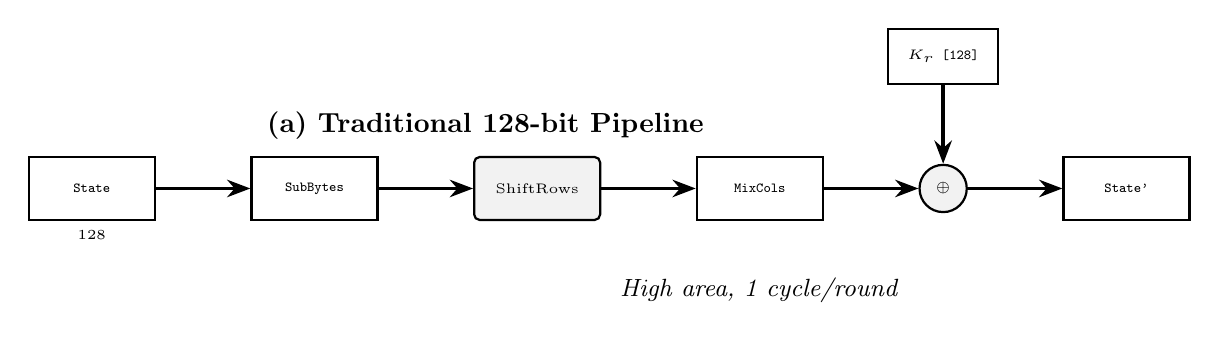
\begin{tikzpicture}[node distance=1cm and 1.2cm]

\node[font=\normalsize\bfseries] at (5,0.8) {(a) Traditional 128-bit Pipeline};

\node[register, minimum width=1.6cm, minimum height=0.8cm] (s0) at (0,0) {State};
\node[register, minimum width=1.6cm, minimum height=0.8cm, right=of s0] (sb) {SubBytes};
\node[logic, right=of sb, minimum width=1.6cm, minimum height=0.8cm] (sr) {ShiftRows};
\node[register, minimum width=1.6cm, minimum height=0.8cm, right=of sr] (mc) {MixCols};
\node[logic, circle, minimum size=0.6cm, right=of mc] (xor) {$\oplus$};
\node[register, minimum width=1.6cm, minimum height=0.8cm, right=of xor] (s1) {State'};

\node[register, above=1cm of xor, minimum width=1.4cm] (rk) {$K_r$ [128]};

\draw[bus] (s0) -- (sb);
\draw[bus] (sb) -- (sr);
\draw[bus] (sr) -- (mc);
\draw[bus] (mc) -- (xor);
\draw[bus] (xor) -- (s1);
\draw[bus] (rk) -- (xor);

\node[buswidth, below=0.1cm of s0.south] {128};
\node[font=\small, below=0.6cm of mc] {\textit{High area, 1 cycle/round}};

\end{tikzpicture}
\end{subfigure}

\vspace{1.5cm}

\begin{subfigure}[b]{0.95\textwidth}
\centering
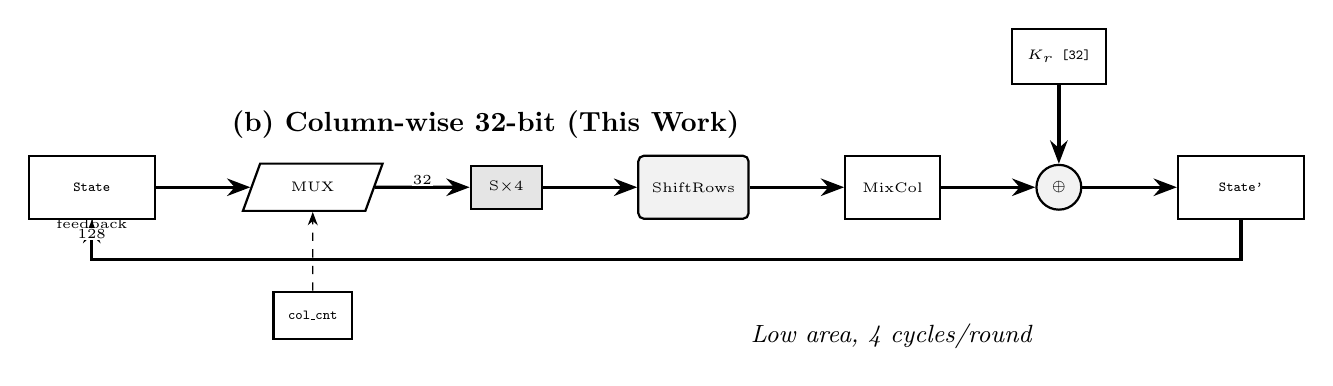
\begin{tikzpicture}[node distance=1cm and 1.2cm]

\node[font=\normalsize\bfseries] at (5,0.8) {(b) Column-wise 32-bit (This Work)};

\node[register, minimum width=1.6cm, minimum height=0.8cm] (s0) at (0,0) {State};
\node[mux, right=of s0, minimum width=1cm] (mux) {MUX};
\node[sbox, right=of mux, minimum width=0.9cm] (sb) {S$\times$4};
\node[logic, right=of sb, minimum width=1.4cm, minimum height=0.8cm] (sr) {ShiftRows};
\node[alu, right=of sr, minimum width=1.2cm, minimum height=0.8cm] (mc) {MixCol};
\node[logic, circle, minimum size=0.55cm, right=of mc] (xor) {$\oplus$};
\node[register, minimum width=1.6cm, minimum height=0.8cm, right=of xor] (s1) {State'};

\node[register, above=1cm of xor, minimum width=1.2cm] (rk) {$K_r$ [32]};
\node[register, below=1cm of mux, minimum width=1cm, minimum height=0.6cm] (cnt) {col\_cnt};

\draw[bus] (s0) -- (mux);
\draw[bus] (mux) -- node[buswidth, above] {32} (sb);
\draw[bus] (sb) -- (sr);
\draw[bus] (sr) -- (mc);
\draw[bus] (mc) -- (xor);
\draw[bus] (xor) -- (s1);
\draw[bus] (rk) -- (xor);
\draw[bus] (s1.south) -- ++(0,-0.5) -| node[near end, above, font=\tiny] {feedback} (s0.south);
\draw[controlwire] (cnt) -- (mux);

\node[buswidth, below=0.1cm of s0.south] {128};
\node[font=\small, below=1.2cm of mc] {\textit{Low area, 4 cycles/round}};

\end{tikzpicture}
\end{subfigure}

\vspace{0.3cm}
\caption{Pipeline comparison: (a) full-width vs (b) column-wise processing.}
\label{fig:pipeline}
\end{figure*}

\clearpage

%==============================================================================
% Figure 3: Key Expansion - IMPROVED SPACING
%==============================================================================
\begin{figure}[!t]
\centering
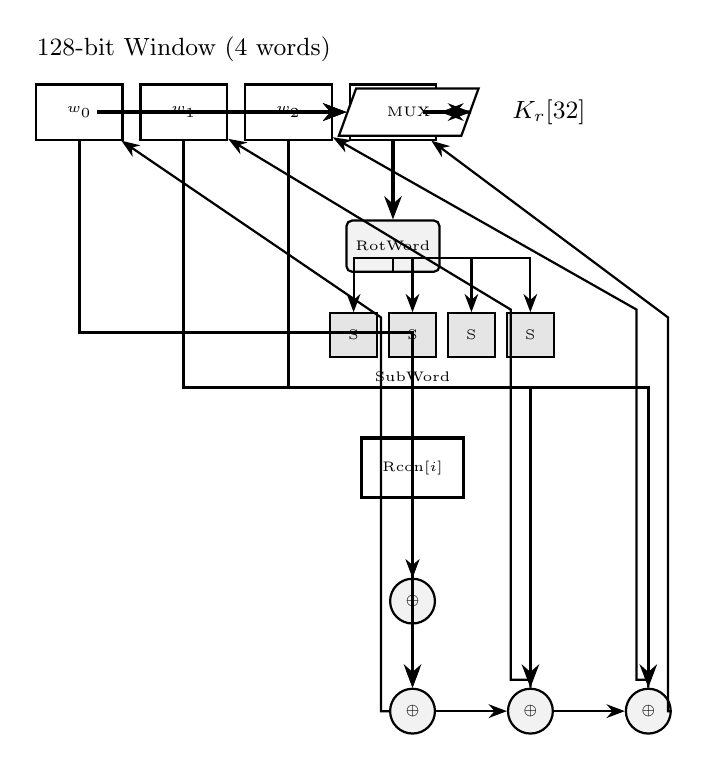
\begin{tikzpicture}[node distance=0.8cm and 1cm]

% Key word registers
\node[register, minimum width=1.1cm, minimum height=0.7cm] (w0) at (0,0) {$w_0$};
\node[register, minimum width=1.1cm, minimum height=0.7cm, right=0.2cm of w0] (w1) {$w_1$};
\node[register, minimum width=1.1cm, minimum height=0.7cm, right=0.2cm of w1] (w2) {$w_2$};
\node[register, minimum width=1.1cm, minimum height=0.7cm, right=0.2cm of w2] (w3) {$w_3$};

\node[font=\small, above=0.15cm of w1.north] {128-bit Window (4 words)};

% RotWord
\node[logic, below=1cm of w3, minimum width=1.1cm, minimum height=0.65cm] (rot) {RotWord};

% SubWord S-boxes
\node[sbox, below=0.5cm of rot, minimum width=0.6cm, xshift=-0.5cm] (s0) {S};
\node[sbox, right=0.12cm of s0, minimum width=0.6cm] (s1) {S};
\node[sbox, right=0.12cm of s1, minimum width=0.6cm] (s2) {S};
\node[sbox, right=0.12cm of s2, minimum width=0.6cm] (s3) {S};
\node[font=\tiny, below=0.05cm of s1.south] {SubWord};

% Rcon
\node[memory, below=1cm of s1, minimum width=1.3cm, minimum height=0.75cm] (rcon) {Rcon[$i$]};

% XOR chain
\node[logic, circle, minimum size=0.5cm, below=1cm of rcon] (x1) {$\oplus$};
\node[logic, circle, minimum size=0.5cm, below=0.8cm of x1] (x2) {$\oplus$};
\node[logic, circle, minimum size=0.5cm, right=0.9cm of x2] (x3) {$\oplus$};
\node[logic, circle, minimum size=0.5cm, right=0.9cm of x3] (x4) {$\oplus$};

% Connections - RotWord and SubWord
\draw[bus] (w3) -- (rot);
\draw[wire] (rot) -- ++(0,-0.15) -| (s0);
\draw[wire] (rot) -- ++(0,-0.15) -| (s1);
\draw[wire] (rot) -- ++(0,-0.15) -| (s2);
\draw[wire] (rot) -- ++(0,-0.15) -| (s3);

% XOR chain connections
\draw[wire] (s1) -- ++(0,-0.3) -| (x1);
\draw[wire] (rcon) -- (x1);
\draw[bus] (w0) -- ++(0,-2.8) -| (x2);
\draw[wire] (x1) -- (x2);
\draw[wire] (x2) -- (x3);
\draw[bus] (w1) -- ++(0,-3.5) -| (x3);
\draw[bus] (w2) -- ++(0,-3.5) -| (x4);
\draw[wire] (x3) -- (x4);

% Feedback paths (new words)
\draw[wire] (x2) -- ++(-0.4,0) -- ++(0,5) -- (w0);
\draw[wire] (x3) -- ++(0,0.4) -- ++(-0.25,0) -- ++(0,4.7) -- (w1);
\draw[wire] (x4) -- ++(0,0.4) -- ++(-0.15,0) -- ++(0,4.7) -- (w2);
\draw[wire] (x4) -- ++(0.25,0) -- ++(0,5) -- (w3);

% Output MUX
\node[mux, right=1.5cm of w1, minimum width=0.9cm] (outmux) {MUX};
\draw[bus] (w0) -- ++(0.25,0) |- (outmux);
\draw[bus] (w1) -- ++(0.3,0) |- (outmux);
\draw[bus] (w2) -- ++(0.35,0) |- (outmux);
\draw[bus] (w3) -- ++(0.4,0) |- (outmux);
\node[right=0.4cm of outmux, font=\small] {$K_r$[32]};
\draw[bus] (outmux) -- ++(0.4,0);

\end{tikzpicture}
\vspace{0.3cm}
\caption{On-the-fly key expansion with 4-word window (90\% memory reduction).}
\label{fig:keyexp}
\end{figure}

\clearpage

%==============================================================================
% Figure 4: SubBytes - IMPROVED LAYOUT
%==============================================================================
\begin{figure}[!t]
\centering
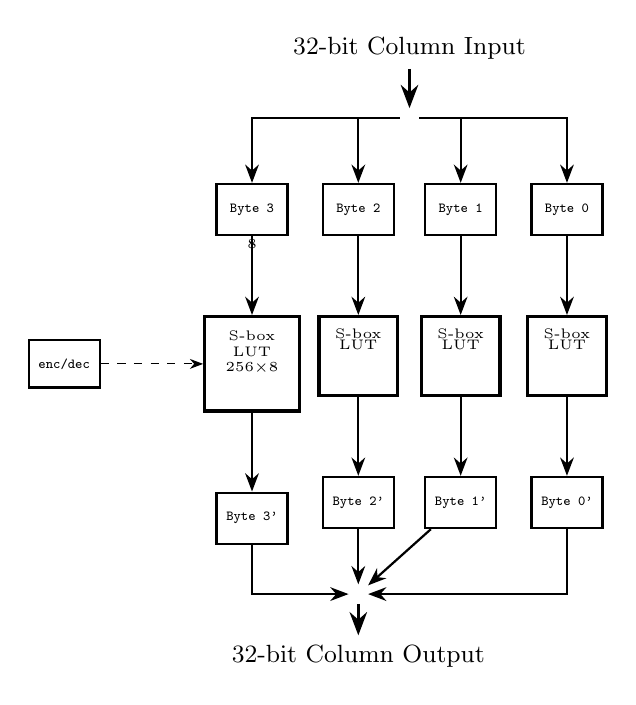
\begin{tikzpicture}[node distance=0.8cm]

\node[font=\small] (in) {32-bit Column Input};
\node[below=0.5cm of in] (split) {};

% Byte extraction
\node[register, below=0.7cm of split, xshift=-2cm, minimum width=0.9cm, minimum height=0.65cm] (b0) {Byte 3};
\node[register, below=0.7cm of split, xshift=-0.65cm, minimum width=0.9cm, minimum height=0.65cm] (b1) {Byte 2};
\node[register, below=0.7cm of split, xshift=0.65cm, minimum width=0.9cm, minimum height=0.65cm] (b2) {Byte 1};
\node[register, below=0.7cm of split, xshift=2cm, minimum width=0.9cm, minimum height=0.65cm] (b3) {Byte 0};

\node[buswidth, below=0.02cm of b0.south] {8};

\draw[bus] (in) -- (split);
\draw[wire] (split) -| (b0);
\draw[wire] (split) -| (b1);
\draw[wire] (split) -| (b2);
\draw[wire] (split) -| (b3);

% S-box LUTs
\node[memory, below=1cm of b0, minimum width=1.2cm, minimum height=1.2cm] (sb0) {};
\node[font=\tiny, below=0.08cm of sb0.north] {S-box};
\node[font=\tiny, below=0.28cm of sb0.north] {LUT};
\node[font=\tiny, below=0.48cm of sb0.north] {256$\times$8};

\node[memory, below=1cm of b1, minimum width=1cm, minimum height=1cm] (sb1) {};
\node[font=\tiny, below=0.05cm of sb1.north] {S-box};
\node[font=\tiny, below=0.2cm of sb1.north] {LUT};

\node[memory, below=1cm of b2, minimum width=1cm, minimum height=1cm] (sb2) {};
\node[font=\tiny, below=0.05cm of sb2.north] {S-box};
\node[font=\tiny, below=0.2cm of sb2.north] {LUT};

\node[memory, below=1cm of b3, minimum width=1cm, minimum height=1cm] (sb3) {};
\node[font=\tiny, below=0.05cm of sb3.north] {S-box};
\node[font=\tiny, below=0.2cm of sb3.north] {LUT};

\draw[wire] (b0) -- (sb0);
\draw[wire] (b1) -- (sb1);
\draw[wire] (b2) -- (sb2);
\draw[wire] (b3) -- (sb3);

% Output bytes
\node[register, below=1cm of sb0, minimum width=0.9cm, minimum height=0.65cm] (o0) {Byte 3'};
\node[register, below=1cm of sb1, minimum width=0.9cm, minimum height=0.65cm] (o1) {Byte 2'};
\node[register, below=1cm of sb2, minimum width=0.9cm, minimum height=0.65cm] (o2) {Byte 1'};
\node[register, below=1cm of sb3, minimum width=0.9cm, minimum height=0.65cm] (o3) {Byte 0'};

\draw[wire] (sb0) -- (o0);
\draw[wire] (sb1) -- (o1);
\draw[wire] (sb2) -- (o2);
\draw[wire] (sb3) -- (o3);

% Merge
\node[below=0.7cm of o1] (merge) {};
\node[font=\small, below=0.4cm of merge] (out) {32-bit Column Output};

\draw[wire] (o0) |- (merge);
\draw[wire] (o1) -- (merge);
\draw[wire] (o2) -- (merge);
\draw[wire] (o3) |- (merge);
\draw[bus] (merge) -- (out);

% Mode control
\node[register, left=1.3cm of sb0, minimum width=0.9cm, minimum height=0.6cm] (mode) {enc/dec};
\draw[controlwire] (mode) -- (sb0.west);

\end{tikzpicture}
\vspace{0.3cm}
\caption{SubBytes with four parallel 256$\times$8 S-box LUTs for 32-bit processing.}
\label{fig:subbytes}
\end{figure}

\clearpage

%==============================================================================
% Figure 5: MixColumns - IMPROVED LAYOUT
%==============================================================================
\begin{figure}[!t]
\centering
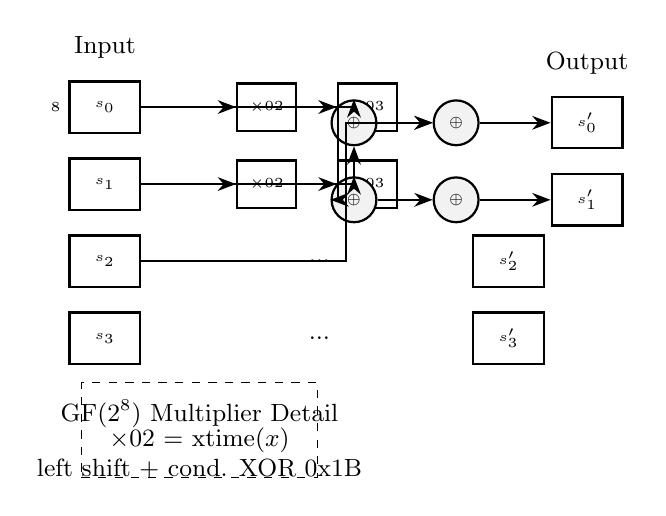
\begin{tikzpicture}[node distance=0.7cm and 0.9cm]

% Input bytes
\node[register, minimum width=0.9cm, minimum height=0.65cm] (s0) at (0,0) {$s_0$};
\node[register, minimum width=0.9cm, minimum height=0.65cm, below=0.3cm of s0] (s1) {$s_1$};
\node[register, minimum width=0.9cm, minimum height=0.65cm, below=0.3cm of s1] (s2) {$s_2$};
\node[register, minimum width=0.9cm, minimum height=0.65cm, below=0.3cm of s2] (s3) {$s_3$};

\node[font=\small, above=0.15cm of s0] {Input};
\node[buswidth, left=0.08cm of s0] {8};

% GF multipliers (showing first two rows)
\node[alu, right=1.2cm of s0, minimum width=0.75cm, minimum height=0.6cm] (m02_0) {$\times$02};
\node[alu, right=0.5cm of m02_0, minimum width=0.75cm, minimum height=0.6cm] (m03_0) {$\times$03};

\node[alu, right=1.2cm of s1, minimum width=0.75cm, minimum height=0.6cm] (m02_1) {$\times$02};
\node[alu, right=0.5cm of m02_1, minimum width=0.75cm, minimum height=0.6cm] (m03_1) {$\times$03};

\draw[wire] (s0) -- (m02_0);
\draw[wire] (s0.east) -- ++(0.4,0) |- (m03_0);
\draw[wire] (s1) -- (m02_1);
\draw[wire] (s1.east) -- ++(0.4,0) |- (m03_1);

% XOR trees (first two outputs)
\node[logic, circle, minimum size=0.5cm, right=2.4cm of s0, yshift=-0.2cm] (x0a) {$\oplus$};
\node[logic, circle, minimum size=0.5cm, right=0.7cm of x0a] (x0b) {$\oplus$};

\node[logic, circle, minimum size=0.5cm, right=2.4cm of s1, yshift=-0.2cm] (x1a) {$\oplus$};
\node[logic, circle, minimum size=0.5cm, right=0.7cm of x1a] (x1b) {$\oplus$};

\draw[wire] (m02_0) -| (x0a);
\draw[wire] (m03_1) -| (x0a);
\draw[wire] (x0a) -- (x0b);
\draw[wire] (s2.east) -- ++(2.6,0) |- (x0b);

\draw[wire] (m02_1) -| (x1a);
\draw[wire] (s0.east) -- ++(2.5,0) |- (x1a);
\draw[wire] (x1a) -- (x1b);

% Output bytes
\node[register, right=0.9cm of x0b, minimum width=0.9cm, minimum height=0.65cm] (o0) {$s_0'$};
\node[register, right=0.9cm of x1b, minimum width=0.9cm, minimum height=0.65cm] (o1) {$s_1'$};
\node[register, right=4.2cm of s2, minimum width=0.9cm, minimum height=0.65cm] (o2) {$s_2'$};
\node[register, right=4.2cm of s3, minimum width=0.9cm, minimum height=0.65cm] (o3) {$s_3'$};

\draw[wire] (x0b) -- (o0);
\draw[wire] (x1b) -- (o1);

\node[font=\small, right=2cm of s2] {...};
\node[font=\small, right=2cm of s3] {...};

\node[font=\small, above=0.15cm of o0] {Output};

% GF multiplier detail box
\node[draw, dashed, below=1.2cm of s2, minimum width=3cm, minimum height=1.2cm, xshift=1.2cm] (detail) {};
\node[font=\small, below=0.1cm of detail.north] {GF($2^8$) Multiplier Detail};
\node[font=\small, below=0.45cm of detail.north, align=center] {$\times$02 = xtime($x$)\\left shift + cond. XOR 0x1B};

\end{tikzpicture}
\vspace{0.3cm}
\caption{MixColumns with GF($2^8$) multipliers and XOR trees for one column.}
\label{fig:mixcol}
\end{figure}

\clearpage

%==============================================================================
% Figure 6: Control FSM - IMPROVED LAYOUT
%==============================================================================
\begin{figure}[!t]
\centering
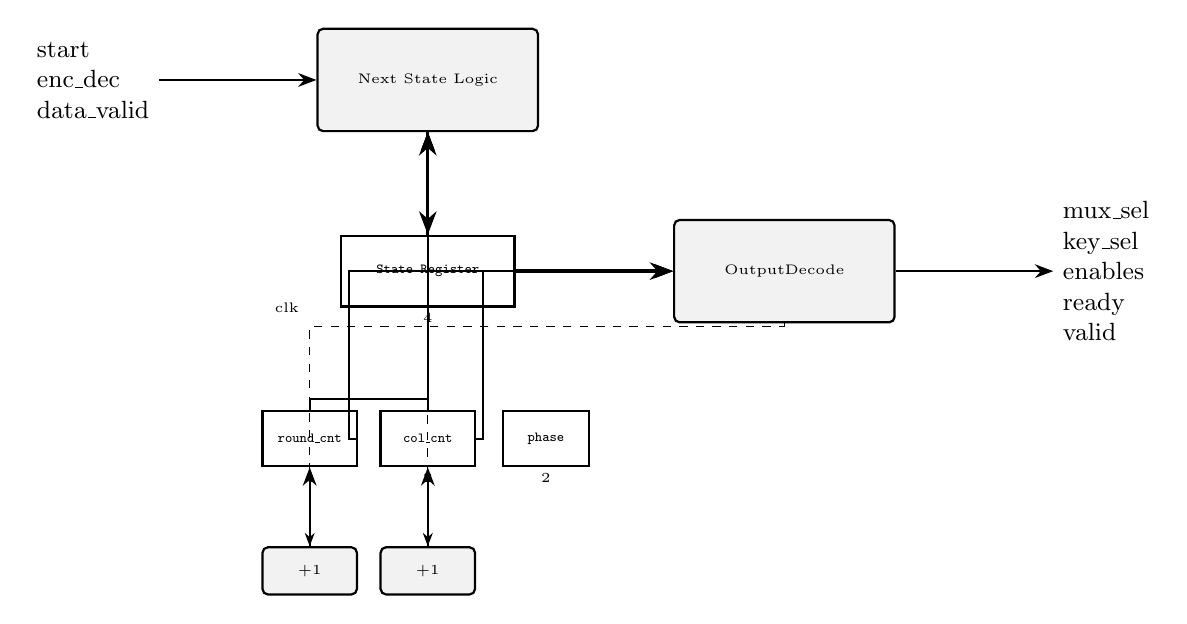
\begin{tikzpicture}[node distance=1cm and 1.5cm]

% State register (center)
\node[register, minimum width=2.2cm, minimum height=0.9cm] (state) at (0,0) {State Register};
\node[buswidth, below=0.05cm of state.south] {4};
\node[font=\tiny, left=0.4cm of state.south west] {clk};

% Next state logic (above)
\node[logic, above=1.3cm of state, minimum width=2.8cm, minimum height=1.3cm] (nsl) {Next State Logic};

% Output/decode logic (right)
\node[logic, right=2cm of state, minimum width=2.8cm, minimum height=1.3cm] (out) {Output\\Decode};

% Counters (below state)
\node[register, below=1.3cm of state, xshift=-1.5cm, minimum width=1.2cm, minimum height=0.7cm] (rc) {round\_cnt};
\node[buswidth, below=0.05cm of rc.south] {4};

\node[register, below=1.3cm of state, xshift=0cm, minimum width=1.2cm, minimum height=0.7cm] (cc) {col\_cnt};
\node[buswidth, below=0.05cm of cc.south] {2};

\node[register, below=1.3cm of state, xshift=1.5cm, minimum width=1.1cm, minimum height=0.7cm] (ph) {phase};
\node[buswidth, below=0.05cm of ph.south] {2};

% Increment logic
\node[logic, below=1cm of rc, minimum width=1.2cm, minimum height=0.6cm] (inc1) {+1};
\node[logic, below=1cm of cc, minimum width=1.2cm, minimum height=0.6cm] (inc2) {+1};

% External inputs (left)
\node[left=2cm of nsl, font=\small, align=left] (inputs) {start\\enc\_dec\\data\_valid};

% Control outputs (right)
\node[right=2cm of out, font=\small, align=left] (outputs) {mux\_sel\\key\_sel\\enables\\ready\\valid};

% Dataflow connections
\draw[bus] (state) -- (nsl);
\draw[bus] (nsl) -- (state);
\draw[bus] (state) -- (out);

\draw[wire] (rc) -- ++(0,0.5) -| (nsl);
\draw[wire] (cc) -- ++(0,0.7) -| (nsl);
\draw[wire] (rc) -- ++(0.5,0) |- (out);
\draw[wire] (cc) -- ++(0.7,0) |- (out);

% Counter control
\draw[controlwire] (out) -- ++(0,-0.7) -| (inc1.north);
\draw[controlwire] (out) -- ++(0,-0.7) -| (inc2.north);
\draw[wire] (inc1) -- (rc);
\draw[wire] (inc2) -- (cc);

% External connections
\draw[wire] (inputs) -- (nsl);
\draw[wire] (out) -- (outputs);

\end{tikzpicture}
\vspace{0.3cm}
\caption{Control FSM with state register, logic blocks, and counters.}
\label{fig:fsm}
\end{figure}

\end{document}
